\fancyhf{}
\setlength{\headheight}{14.49998pt}
\lhead{\textsl{\footnotesize{\nouppercase{\rightmark}}}}
\rhead{\textsl{\footnotesize{\nouppercase{\leftmark}}}}

\cfoot{\thepage}
\rfoot{\textsl{\footnotesize}}

\chapter{Requirement Analysis and Project Scope}

\section{Introduction}
This chapter formalizes the analytical foundation of the project by translating the initial problem context into explicit system expectations. It clarifies who interacts with the solution, what behaviors the system must provide, and which quality properties must be preserved during operation. The analysis is supported by UML\footnote{\textit{Unified Modeling Language}.} modeling to represent interactions, process flow, and message exchange dynamics in a structured and verifiable way.

It also defines the practical boundaries of the work by separating what the project intentionally addresses from what remains outside the current implementation perimeter, while stating the main constraints and working assumptions that influenced design choices. Establishing these elements at this stage is essential: it reduces ambiguity, aligns technical development with business objectives, and provides a traceable reference for architecture, implementation, and validation decisions in the next chapters.

\section{Functional Requirements}
Functional requirements describe what the chatbot must concretely do from the user's point of view during a real commercial conversation.

\begin{enumerate}
    \item \textbf{FR-01 --- Multi-platform availability:} the chatbot must operate on Facebook Messenger, Instagram, and WhatsApp with a consistent interaction experience across the three channels.
    \item \textbf{FR-02 --- Inquiry handling and need identification:} the chatbot must understand the user's intent, identify their needs, and provide relevant answers to their questions throughout the conversation.
    \item \textbf{FR-03 --- Language-adaptive understandable responses:} the chatbot must provide understandable answers in the user's language, with responses configured primarily in French or Tunisian dialect according to conversation context.
    \item \textbf{FR-04 --- Approximate quote generation:} the chatbot must be able to collect essential customer information and produce an approximate commercial quote.
    \item \textbf{FR-05 --- Human handoff behavior:} when the user explicitly asks to speak with a human, the chatbot must stop automated interaction and defer the conversation to a human agent.
    \item \textbf{FR-06 --- Conversation memory:} the chatbot must preserve user-specific conversation history so that exchanges remain coherent over multiple messages.
    \item \textbf{FR-07 --- Identity transparency:} the chatbot must clearly behave as an AI assistant and must not present itself as a human representative.
\end{enumerate}

\section{Non-Functional Requirements}
Non-functional requirements define the quality constraints under which the previous functionalities must be delivered.

\begin{enumerate}
    \item \textbf{NFR-01 --- Response time:} the chatbot should respond quickly, with a target upper bound of 30 seconds for a complete answer in normal operating conditions.
    \item \textbf{NFR-02 --- Security and confidentiality:} the chatbot must protect sensitive internal information and must never reveal confidential elements such as system-level instructions.
    \item \textbf{NFR-03 --- Resilience and service continuity:} the chatbot should remain stable under common failures or unexpected inputs and continue providing safe, controlled behavior.
\end{enumerate}

\section{Identification of Actors}
The chatbot ecosystem involves three primary actors whose interactions define the operational behavior of the system:

\begin{enumerate}
    \item \textbf{User:} the external customer who initiates the conversation, requests service information, asks technical or commercial questions, and seeks an approximate quote.
    \item \textbf{Commercial Agent:} the human sales representative who takes over the conversation when human assistance is requested and continues the commercial follow-up process.
    \item \textbf{System Administrator:} the internal actor responsible for configuring, supervising, and maintaining the chatbot environment, including behavior rules, security settings, and operational continuity.
\end{enumerate}

Together, these actors delimit the functional interaction perimeter analyzed in the rest of the chapter and provide the reference frame for UML modeling in the following sections.

\section{Use Case Diagram}
The use case diagram synthesizes the functional interaction view of the chatbot by mapping each actor to the goals they pursue through the system. It highlights user-facing goals (information request, quote request, and human assistance), operational commercial actions, and administrative control tasks, while preserving a clear boundary around the chatbot platform.

\begin{figure}[H]
    \centering
    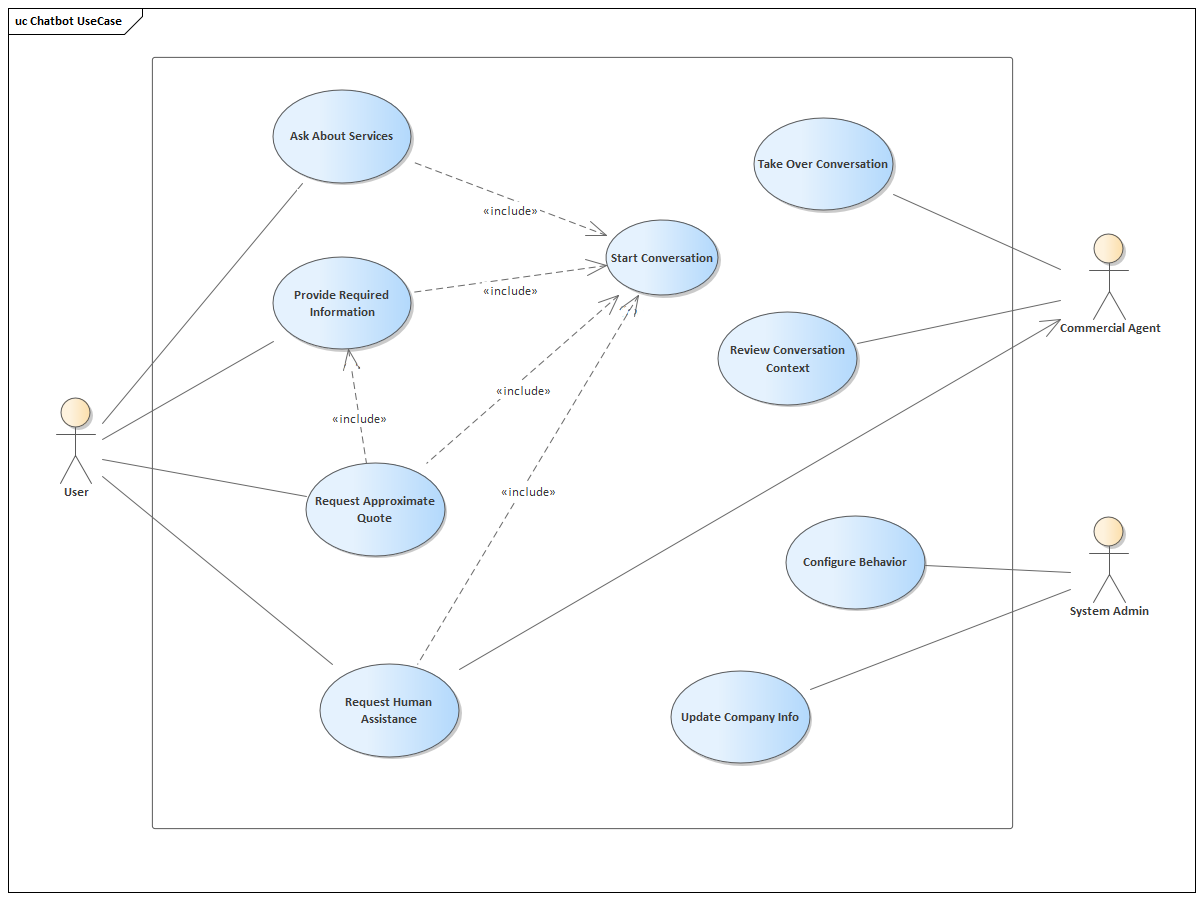
\includegraphics[width=0.95\textwidth]{Images/diagrams/usecase_diagram.png}
    \caption{Use case diagram of the Sparky AI commercial chatbot system.}
    \label{fig:usecase-diagram}
\end{figure}

\section{Textual Description of Use Case Diagram}
To complement the graphical representation, each use case is specified below with a structured textual template. This description formalizes execution conditions and expected outcomes, and serves as a precise reference for implementation and validation activities.

\noindent The first use case captures how a customer initiates interaction with the chatbot.
\begin{table}[H]
\centering
\caption{Use case specification: Start Conversation}
\label{tab:uc-start-conversation}
\begin{tabular}{|p{0.25\textwidth}|p{0.64\textwidth}|}
\hline
\textbf{Title} & Start Conversation \\
\hline
\textbf{Main Actor} & User \\
\hline
\textbf{Description} & The user initiates a new conversation session with the chatbot through one of the supported channels. \\
\hline
\textbf{Pre-conditions} & The user has access to a supported messaging channel and the chatbot service is available. \\
\hline
\textbf{Post-conditions} & A conversation session is initialized and ready for subsequent user requests. \\
\hline
\textbf{Nominal scenario} & 1. The user sends an initial message. \newline 2. The chatbot receives and acknowledges the message. \newline 3. The chatbot returns an opening response and waits for the user's next intent. \\
\hline
\end{tabular}
\end{table}

\noindent The following use case describes how the user requests general business information.
\begin{table}[H]
\centering
\caption{Use case specification: Ask About Services}
\label{tab:uc-ask-about-services}
\begin{tabular}{|p{0.25\textwidth}|p{0.64\textwidth}|}
\hline
\textbf{Title} & Ask About Services \\
\hline
\textbf{Main Actor} & User \\
\hline
\textbf{Description} & The user asks questions about available products, services, or commercial offerings. \\
\hline
\textbf{Pre-conditions} & A conversation has already started. \\
\hline
\textbf{Post-conditions} & The user receives relevant service-related information. \\
\hline
\textbf{Nominal scenario} & 1. The user asks about a service. \newline 2. The chatbot interprets the request. \newline 3. The chatbot provides a targeted informational response. \newline 4. The user may continue with follow-up questions. \\
\hline
\end{tabular}
\end{table}

\noindent The next use case formalizes the customer input phase needed for commercial qualification.
\begin{table}[H]
\centering
\caption{Use case specification: Provide Required Information}
\label{tab:uc-provide-required-information}
\begin{tabular}{|p{0.25\textwidth}|p{0.64\textwidth}|}
\hline
\textbf{Title} & Provide Required Information \\
\hline
\textbf{Main Actor} & User \\
\hline
\textbf{Description} & The user submits required project and profile information requested by the chatbot. \\
\hline
\textbf{Pre-conditions} & The conversation is active and the chatbot has requested specific data elements. \\
\hline
\textbf{Post-conditions} & Required inputs are captured in conversation context for subsequent processing. \\
\hline
\textbf{Nominal scenario} & 1. The chatbot asks for required details. \newline 2. The user provides requested information. \newline 3. The chatbot validates completion and confirms receipt. \\
\hline
\end{tabular}
\end{table}

\noindent The following use case describes the quote-oriented interaction objective.
\begin{table}[H]
\centering
\caption{Use case specification: Request Approximate Quote}
\label{tab:uc-request-approximate-quote}
\begin{tabular}{|p{0.25\textwidth}|p{0.64\textwidth}|}
\hline
\textbf{Title} & Request Approximate Quote \\
\hline
\textbf{Main Actor} & User \\
\hline
\textbf{Description} & The user requests an approximate quotation based on available project information. \\
\hline
\textbf{Pre-conditions} & The conversation is active and at least minimal qualification data is available or can be requested. \\
\hline
\textbf{Post-conditions} & An approximate quote is delivered, or missing information is explicitly requested. \\
\hline
\textbf{Nominal scenario} & 1. The user asks for a quote. \newline 2. The chatbot checks available inputs. \newline 3. If necessary, the chatbot requests additional details. \newline 4. The chatbot returns an approximate commercial estimate. \\
\hline
\end{tabular}
\end{table}

\noindent The next use case captures escalation from automated interaction to human follow-up.
\begin{table}[H]
\centering
\caption{Use case specification: Request Human Assistance}
\label{tab:uc-request-human-assistance}
\begin{tabular}{|p{0.25\textwidth}|p{0.64\textwidth}|}
\hline
\textbf{Title} & Request Human Assistance \\
\hline
\textbf{Main Actor} & User \\
\hline
\textbf{Description} & The user explicitly requests to continue the interaction with a human commercial representative. \\
\hline
\textbf{Pre-conditions} & An active conversation exists between the user and the chatbot. \\
\hline
\textbf{Post-conditions} & The conversation is marked for human takeover and chatbot auto-replies are suspended according to policy. \\
\hline
\textbf{Nominal scenario} & 1. The user requests a human agent. \newline 2. The chatbot acknowledges the request. \newline 3. The chatbot triggers handoff state and informs the user that a commercial agent will continue. \\
\hline
\end{tabular}
\end{table}

\noindent The following use case defines the commercial agent intervention phase.
\begin{table}[H]
\centering
\caption{Use case specification: Take Over Conversation}
\label{tab:uc-take-over-conversation}
\begin{tabular}{|p{0.25\textwidth}|p{0.64\textwidth}|}
\hline
\textbf{Title} & Take Over Conversation \\
\hline
\textbf{Main Actor} & Commercial Agent \\
\hline
\textbf{Description} & The commercial agent assumes direct control of a conversation after handoff is requested. \\
\hline
\textbf{Pre-conditions} & A valid handoff request exists for the target conversation. \\
\hline
\textbf{Post-conditions} & Human-led interaction is active and the user is handled directly by the commercial agent. \\
\hline
\textbf{Nominal scenario} & 1. The agent receives handoff notification. \newline 2. The agent opens the corresponding conversation. \newline 3. The agent sends the first human response and continues commercial discussion. \\
\hline
\end{tabular}
\end{table}

\noindent The next use case specifies how the agent prepares for an informed takeover.
\begin{table}[H]
\centering
\caption{Use case specification: Review Conversation Context}
\label{tab:uc-review-conversation-context}
\begin{tabular}{|p{0.25\textwidth}|p{0.64\textwidth}|}
\hline
\textbf{Title} & Review Conversation Context \\
\hline
\textbf{Main Actor} & Commercial Agent \\
\hline
\textbf{Description} & The commercial agent reviews prior chatbot-user exchanges before continuing the conversation. \\
\hline
\textbf{Pre-conditions} & Conversation history is available and accessible to the commercial agent. \\
\hline
\textbf{Post-conditions} & The agent has sufficient context to continue discussion without requesting redundant information. \\
\hline
\textbf{Nominal scenario} & 1. The agent opens the conversation record. \newline 2. The agent reads relevant past messages. \newline 3. The agent identifies user needs and pending topics. \newline 4. The agent proceeds with targeted follow-up. \\
\hline
\end{tabular}
\end{table}

\noindent The following use case defines administrative control over chatbot behavior.
\begin{table}[H]
\centering
\caption{Use case specification: Configure Behavior}
\label{tab:uc-configure-behavior}
\begin{tabular}{|p{0.25\textwidth}|p{0.64\textwidth}|}
\hline
\textbf{Title} & Configure Behavior \\
\hline
\textbf{Main Actor} & System Administrator \\
\hline
\textbf{Description} & The administrator updates chatbot behavior parameters, operational rules, and guidance logic. \\
\hline
\textbf{Pre-conditions} & The administrator is authenticated and has configuration privileges. \\
\hline
\textbf{Post-conditions} & Updated behavior settings are saved and applied to subsequent chatbot interactions. \\
\hline
\textbf{Nominal scenario} & 1. The administrator accesses configuration controls. \newline 2. The administrator adjusts behavioral settings. \newline 3. The changes are validated and saved. \newline 4. The chatbot operates under the new configuration. \\
\hline
\end{tabular}
\end{table}

\noindent The final use case captures maintenance of business information used in conversations.
\begin{table}[H]
\centering
\caption{Use case specification: Update Company Info}
\label{tab:uc-update-company-info}
\begin{tabular}{|p{0.25\textwidth}|p{0.64\textwidth}|}
\hline
\textbf{Title} & Update Company Info \\
\hline
\textbf{Main Actor} & System Administrator \\
\hline
\textbf{Description} & The administrator updates company data used by the chatbot, such as offerings, constraints, and commercial reference information. \\
\hline
\textbf{Pre-conditions} & The administrator is authenticated and updated company information is available. \\
\hline
\textbf{Post-conditions} & The chatbot references the latest validated company information in future interactions. \\
\hline
\textbf{Nominal scenario} & 1. The administrator opens company information management. \newline 2. The administrator modifies relevant entries. \newline 3. The updates are reviewed and confirmed. \newline 4. The chatbot uses the updated data in responses. \\
\hline
\end{tabular}
\end{table}

\section{Activity Diagram}
The activity diagram presents the dynamic workflow of a standard chatbot interaction, from the user's initial message to response delivery or human handoff. It captures the main control flow, decision points, and operational branches that govern conversational processing.

\begin{figure}[H]
    \centering
    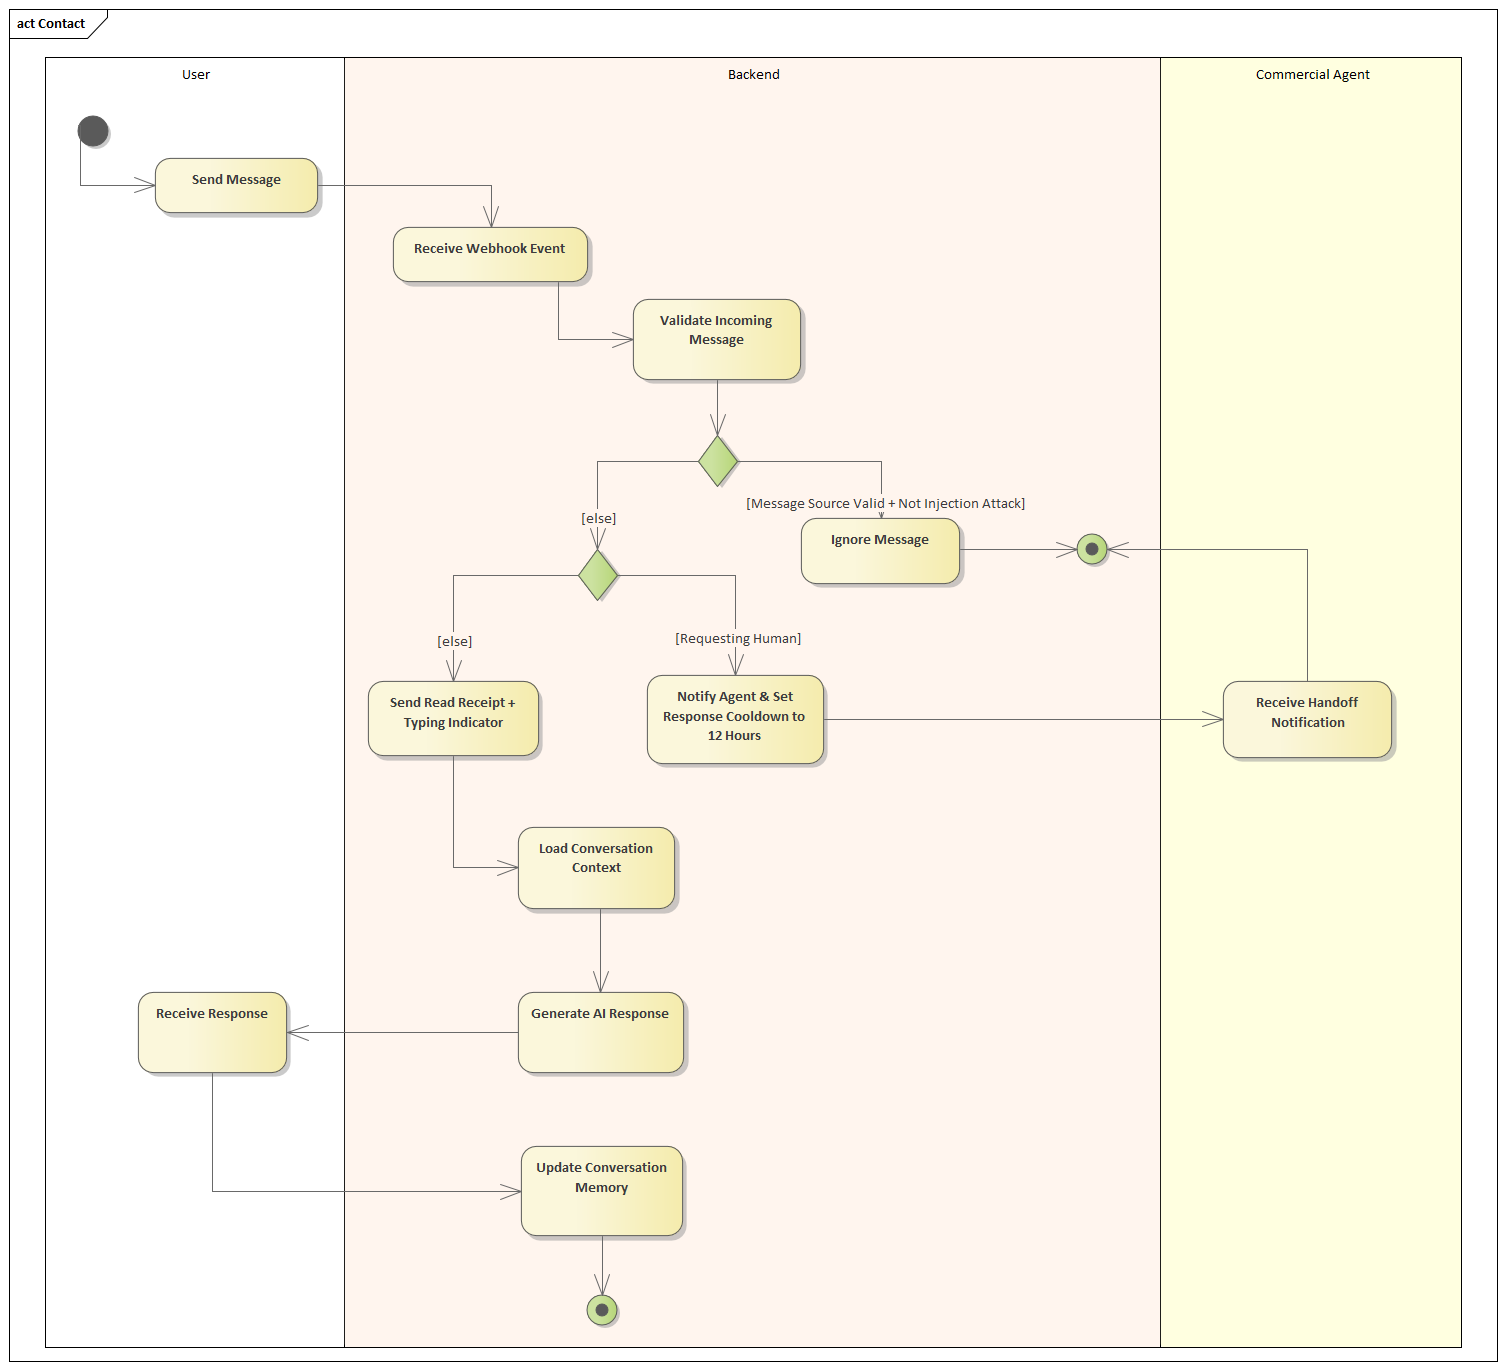
\includegraphics[width=0.95\textwidth]{Images/diagrams/activity_diagram.png}
    \caption{Activity diagram of the Sparky AI chatbot interaction workflow.}
    \label{fig:activity-diagram}
\end{figure}

\section{Project Scope}
The project scope defines the implementation perimeter adopted for this end-of-year work. It clarifies which capabilities are intentionally delivered in the current version of the chatbot and which capabilities are explicitly deferred to future iterations. This delimitation ensures that development effort remains aligned with the chapter requirements, available resources, and the commercial objective of accelerating first customer contact.

\subsection{Scope Boundaries}
The scope boundaries are divided into in-scope and out-of-scope elements.

\subsubsection {In-Scope}
The current project includes the following elements:
\begin{enumerate}
    \item Deployment of a single AI commercial assistant across Facebook Messenger, Instagram, and WhatsApp.
    \item Handling of user inquiries related to Sparky services and customer need qualification.
    \item Generation of approximate commercial quotes based on information provided during the conversation.
    \item Conversation continuity through per-user context memory in multi-turn interaction.
    \item Human handoff behavior when explicitly requested by the user, including chatbot backoff logic.
    \item Administrative control of chatbot behavior and company information updates.
    \item Security guardrails that prevent disclosure of confidential internal instructions.
\end{enumerate}

\subsubsection {Out-of-Scope}
The following elements are outside the scope of this project version:
\begin{enumerate}
    \item Production of legally binding final quotations or automatic contract generation.
    \item Full technical engineering studies (e.g., physical site inspection and installation design validation).
    \item Complete CRM/ERP integration and end-to-end sales pipeline automation.
    \item Autonomous commercial closure without human validation by a commercial agent.
    \item Large-scale model fine-tuning based on proprietary historical datasets.
\end{enumerate}

\section{Constraints and Assumptions}
This part formalizes the main limits under which the solution is designed and the operational hypotheses required for expected behavior in production use.

\subsection{Constraints}
The project is bounded by the following constraints:
\begin{enumerate}
    \item \textbf{Data constraint:} available proprietary conversational data is not sufficient for robust model fine-tuning, which motivates a prompt-engineering and tool-assisted approach.
    \item \textbf{External platform dependency:} message exchange depends on Meta platform services and API policies, including rate limits and webhook behavior.
    \item \textbf{AI service dependency:} response generation quality and latency are partially conditioned by third-party LLM service availability.
    \item \textbf{Operational resource constraint:} the company does not maintain a dedicated social media team, limiting continuous human intervention capacity.
    \item \textbf{Security and compliance constraint:} the chatbot must enforce strict confidentiality of internal instructions and avoid unsafe or policy-violating outputs.
    \item \textbf{Project perimeter constraint:} the delivered version targets pre-sales qualification and approximate estimation, not full commercial process automation.
\end{enumerate}

\subsection{Assumptions}
The following assumptions are adopted for analysis and implementation:
\begin{enumerate}
    \item Users provide sufficiently accurate information to enable meaningful approximate quote generation.
    \item System administrators keep business content and operational settings up to date.
    \item Commercial agents take over conversations in a timely manner when human assistance is requested.
    \item Messaging channels remain available under normal operating conditions during chatbot interaction.
    \item Users understand that the assistant is an AI system and that final commercial validation remains under human responsibility.
\end{enumerate}

\section{Conclusion}
Chapter 2 translated the project context into a structured requirement baseline by defining expected functional behavior, quality constraints, actor roles, and interaction dynamics through UML artifacts. It also clarified the implementation perimeter through explicit in-scope and out-of-scope boundaries, then formalized the main constraints and assumptions governing feasibility and operational reliability.

These elements are critical because they establish a shared and verifiable reference for all subsequent technical decisions. The next chapter, \textit{AI and System Design}, builds on this analytical foundation to present the architecture, integration logic, and model-level design choices that implement the defined requirements.
